\newpage

\section{Piktogrammerkennung}
Im Abschnitt \ref{sec:architecture-feature-matching} wurde die Feature-Matching-Image-Detector-Komponenten bereits vorgestellt. In diesem Kapitel wird speziell auf das im \texttt{SiftImageDetector} Modul implementierte Feature Matchingverfahren mit OpenCV eingegangen. Es wird der Lösungsweg aufgezeigt, wie die Klassifizierungsgenauigkeit und die Laufzeit-Performance optimiert werden kann. Sämtlicher Programmcode welcher in den nachfolgenden Versuchen verwendet wurde ist auf Github \footnote{https://github.com/randombenj/hslu-pren2-doc} im Modul image\_detector zu finden.

\subsection{Übersicht Feature Matching}
Als Feature Matching \cite{feature-matching} wird ein Verfahren bezeichnet, bei welchem aus einem Bild gewisse Merkmale extrahiert werden. Diese können beispielsweise in einer Datenbank abgespeichert werden. Zu einem späteren Zeitpunkt können diese Merkmale mit jenen eines anderen Bildes abgleichen werden. Stimmen eine gewisse Anzahl dieser überein, so stimmen auch die dazugehörigen Teile der beiden Bilder überein. Dieser Vorgang kann in die nachfolgenden drei Teile unterteilt werden.

\begin{enumerate}
    \item Detektion (Extraktion der Merkmale auch Keypoints genannt)
    \item Deskription (Eindeutige Beschreibung der Merkmale)
    \item Matching (Vergleichen der Merkmale)
\end{enumerate}

Für jeden dieser drei Schritte gibt es verschiedene Algorithmen, welche zum Ziel führen. Gängige Detektoren und Deskriptoren sind z.B. SIFT, ORB, SURF oder MSER. Für das Matching bietet sich das Bruteforce Matching oder ein FLANN \cite{flann} basiertes Matching an. 

\subsection{Genauigkeit}
Es wurde festgestellt, dass ab einer gewissen Entfernung des Piktogramms die Anzahl guter Matches stark abnimmt. Es wurde ebenfalls festgestellt, dass falls das Piktogramm herangezoomt wird und somit weniger Hintergrund vorhanden war, die Genauigkeit erhöht wurde. Dies führte zum Schluss, dass grosse Hintergrundflächen die Ergebnisse negativ beeinflussen. Da ein heranzoomen jedoch auch negative Seiten hat bezüglich der Sichtweite wurde versucht, die Region of Interest (ROI) vor der Detektion einzugrenzen. Als erstes wurden jedoch verschiedene Algorithmen für die Detektion und Deskription ausprobiert. Hierbei wurde der Fokus auf SIFT und ORB gelegt. Um den ROI einzugrenzen wurde versucht das Bild für die Detektion in mehrere Teile zu zerlegen. Weiter wurde versucht mithilfe von Histogram Backprojection abzuschätzen, wo sich das Piktogramm in etwa befinden könnte.

\subsubsection{Vergleich SIFT vs. ORB}
\textbf{ORB}\\
Der Vergleich von verschiedenen Feature Matching verfahren im Rahmen einer Masterarbeit \cite{feature-matching-riegler-ma} zeigte, dass ORB deutlich schneller ist als SIFT. Dies gilt sowohl für die Detektion als auch die Deskription. Aus diesem Grund wurde zu Beginn ORB bevorzugt. Die Resultate waren jedoch mit 0 guten Matches (siehe \ref{tab:orb-matchingresultate}) nicht sehr vielversprechend. Im Nachhinein wurde herausgefunden, dass ORB deutlich schlechter mit Skalierung umgehen kann, als die meisten anderen Feature Matching Algorithmen. 

In den nachfolgenden Abbildungen \ref{fig:orb-kp1} und \ref{fig:orb-kp2} sind die extrahierten Merkmale visualisiert. In den darauf folgenden Abbildungen \ref{fig:orb-matches-0.75} und \ref{fig:orb-matches-0.85} sind die Anzahl positiver Matches mit eine Matchverhältnis von 0.75 bzw. 0.85. Ein grösseres Matchverhältnis bedeuted in diesem Fall, dass die Distanz zwischen den Punkten grösser sein darf. Das heisst die Punkte bei einem Verhältnis mit 0.75 müssen sich ähnlicher sein als die Punkte bei einem Verhältnis mit 0.85, um als positiven Match gezählt zu werden. In der Abbildung \ref{fig:orb-matches-0.85} ist ersichtlich, dass das Verhältnis zu grosszügig gewählt wurde, da Punkte welche im Kontext absolut keinen Zusammenhang haben, bereits als positive Matches gewertet werden.

\begin{figure}[H]
  \centering
  \begin{minipage}[t]{0.45\linewidth}
  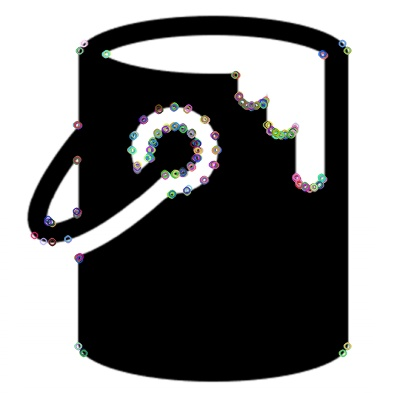
\includegraphics[width=1.0\textwidth]{img/piktogrammerkennung/orb_kp1.jpg}
  \caption{Extrahierte Merkmale mit ORB vom Template}
  \label{fig:orb-kp1}
  \end{minipage} 
  \hfill
  \begin{minipage}[t]{0.45\linewidth}
  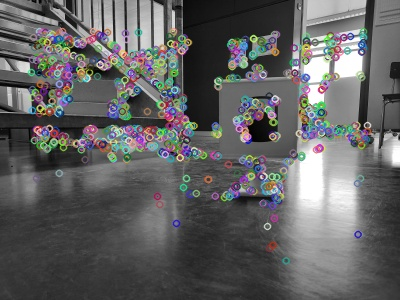
\includegraphics[width=1.0\textwidth]{img/piktogrammerkennung/orb_kp2.jpg}
  \caption{Extrahierte Merkmale mit ORB vom Inputbild}
  \label{fig:orb-kp2}
  \end{minipage}
\end{figure}

\begin{figure}[H]
  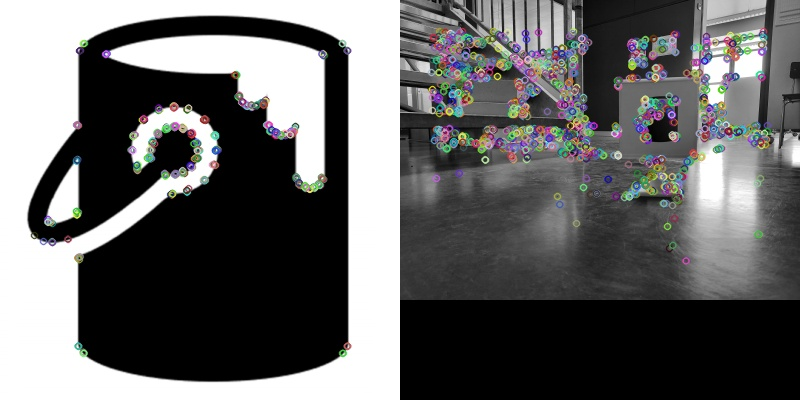
\includegraphics[width=0.95\textwidth]{img/piktogrammerkennung/orb_matches.jpg}
  \centering
  \caption{Matches der ORB Merkmale mit einem Matchverhältniss von 0.75}
  \label{fig:orb-matches-0.75}
\end{figure}

\textbf{Matching Resultate}
\begin{center}
\begin{table}[H]
\begin{tabular}{|l|r|}
\hline
Keypoints 1 & 388 \\
\hline
Keypoints 2 & 1903 \\
\hline
Matches & 388 \\
\hline
Good Matches & 0 \\
\hline
\end{tabular}
\caption[ORB-Matchingresultate mit 0.75 Matchverhältniss]{ORB-Matchingresultate  mit 0.75 Matchverhältniss}
\label{tab:orb-matchingresultate-0.75}
\end{table}
\end{center}

\begin{figure}[H]
  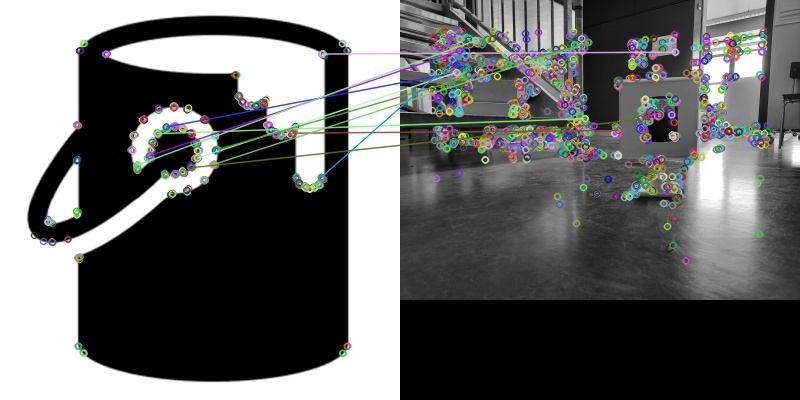
\includegraphics[width=0.95\textwidth]{img/piktogrammerkennung/orb_matches_0.85.jpg}
  \centering
  \caption{Matches der ORB Merkmale mit einem Matchverhältniss von 0.85}
  \label{fig:orb-matches-0.85}
\end{figure}

\textbf{SIFT}\\
SIFT (Scale Invariant Feature Transform) ist einer der bekanntesten Algorithmen für die Merkmalsdetektion. In der Arbeit von Riegler \cite{feature-matching-riegler-ma} beweist er sich als guten Allrounder, schneidet in der Bewertung jedoch nicht sehr gut ab, da er deutlich langsamer als z.B. ORB ist und nicht bemerkenswert bessere Ergebnisse liefert. Da SIFT jedoch deutlich besser mit Skalierung umgehen kann, zeigt er auf der Abbildung \ref{fig:sift-matches-0.7} mit 3 guten Matches bessere Resultate als ORB. Obschon ORB deutlich mehr Keypunkte aus einem Bild extrahiert als SIFT. Es wurde entscheiden die Piktogrammerkennung mit SIFT zu realisieren, da SIFT in den ersten Tests (mit einem grossen Skalierungsfaktor) besser abgeschnitten hat.

\begin{figure}[H]
  \centering
  \begin{minipage}[t]{0.45\linewidth}
  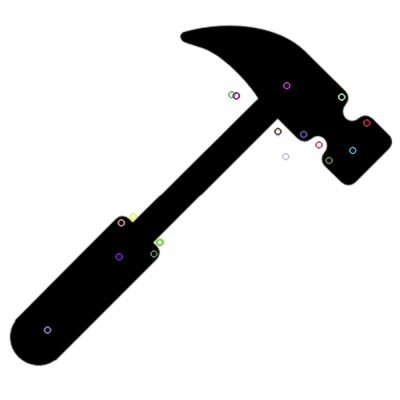
\includegraphics[width=1.0\textwidth]{img/piktogrammerkennung/sift_kp1.jpg}
  \caption{Extrahierte Merkmale mit SIFT vom Template}
  \label{fig:sift-kp1}
  \end{minipage} 
  \hfill
  \begin{minipage}[t]{0.45\linewidth}
  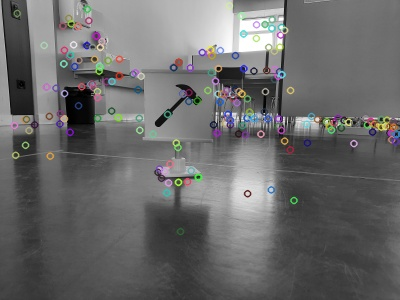
\includegraphics[width=1.0\textwidth]{img/piktogrammerkennung/sift_kp2.jpg}
  \caption{Extrahierte Merkmale mit SIFT vom Inputbild}
  \label{fig:sift-kp2}
  \end{minipage}
\end{figure}

\begin{figure}[H]
  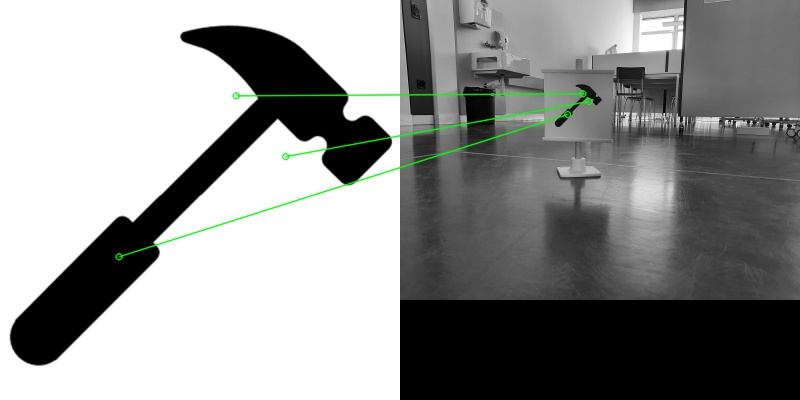
\includegraphics[width=0.95\textwidth]{img/piktogrammerkennung/sift_matches.jpg}
  \centering
  \caption{Matches der SIFT Merkmale mit einem Matchverhältniss von 0.7}
  \label{fig:sift-matches-0.7}
\end{figure}

\textbf{Matching Resultate}
\begin{center}
\begin{table}[H]
\begin{tabular}{|l|r|}
\hline
Keypoints 1 & 31 \\
\hline
Keypoints 2 & 233 \\
\hline
Matches & 31 \\
\hline
Good Matches & 3 \\
\hline
\end{tabular}
\caption[SIFT-Matchingresultate]{SIFT-Matchingresultate}
\label{tab:sift-matchingresultate}
\end{table}
\end{center}

\subsubsection{ROI Eingrenzung mittels Histogramm Backprojection}
Bei der Histogramm Backprojection wird einfach gesagt, ein Bild erzeugt, bei welchem jedes Pixel die Wahrscheinlichkeit angibt, dass es zum vorgegebenen Template gehört. Ist es zu 100\% wahrscheinlich, dass das Pixel im Inputbild zu einem vorgegebenen Template gehört, wird erhält dies beispielsweise den Wert 255. Desto weniger gross die Chance ist, desto kleiner wird der Graustufenwert des Pixels.

Diese resultierende Wahrscheinlichkeitsmatrix kann  mithilfe von Thresholding zu einer Maske verarbeitet werden und mit dem Inputbild multipliziert oder auch bitweise Und-Verknüpfen weden. Somit können die Stellen des Bildes, welche wahrscheinlicher zu einem Template gehören herausfiltern.

Das Ziel war es also, anhand dieser Maske herauszufinden, auf welche Stelle im Inputbild gezoomt werden soll. So wird verhindert, dass aus Versehen die Stelle welche das Piktogramm beinhaltet wegschnitten wird.

Auf dem Bild \ref{fig:backprojection-hammer} sind die drei oben beschriebenen Schritte visualisiert. Ganz links ist das Inputbild zu sehen, in der Mitte die Maske welche sich aus der Wahrscheinlichkeitsmatrix ergeben haben. Ganz rechts ist das Resultat aus der Multiplikation von der Maske mit dem Inputbild zu sehen. Als Template wurde das Piktogramm auf folgender Abbildung \ref{fig:sift-kp1} verwendet. Bereits in der Maske aber vorallem auch im Bild ganz rechts ist zu sehen, dass das Piktogramm nicht erkannt wurde. 

\begin{figure}[H]
  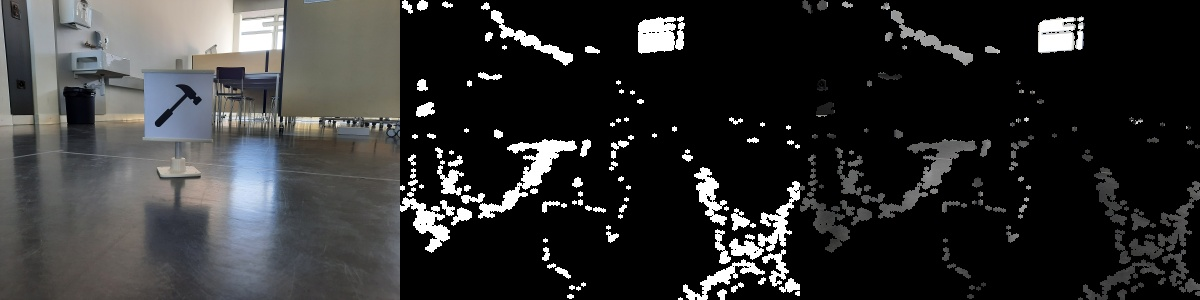
\includegraphics[width=1\textwidth]{img/piktogrammerkennung/hammer_backprojection.jpg}
  \centering
  \caption{Histogramm Backprojection vom Hammer Piktogramm}
  \label{fig:backprojection-hammer}
\end{figure}

Da der selbe Programmcode auf einem anderen Bild viel bessere Resultate erzielte, wurde dieser Ansatz verworfen. Das Bild \ref{fig:backprojection-hand} zeigt, dass der grüne Hintergrund ziemlich gut von den Händen differenziert werden konnten. Ein Grund für die schlechten Ergebnisse mit dem Piktogramm als Template kann sein, dass diese lediglich schwarze und weisse Pixel beinhalten und der Hintergrund des Inputbildes ebenfalls wenig unterschiedliche Farben enthält. Der Algorithmus für die Histogramm Backprojection arbeitet jedoch mit dem HSV-Wert. Somit ist es möglich, dass die HSV-Werte zu wenig grosse Unterschiede aufweisen, als dass diese ohne aufwändiges Finetuneing der Hyperparameter deutlich unterschieden werden können. Wenn jedoch ein grüner Pixel (HSV: 120) von einem Roten Pixel (HSV: 0) unterschieden werden muss, ist dies einfacher, da die Differenz zwischen den HSV-Werten viel deutlicher ist. 

\begin{figure}[H]
  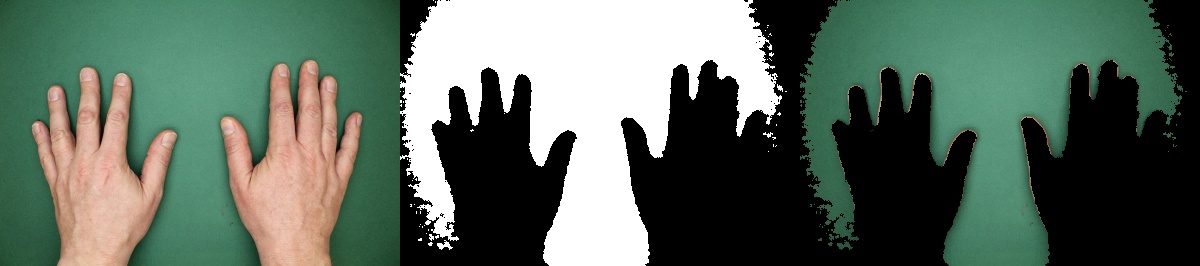
\includegraphics[width=1\textwidth]{img/piktogrammerkennung/hand_backprojection.jpg}
  \centering
  \caption{Histogramm Backprojection vom gut geeignetem Bild}
  \label{fig:backprojection-hand}
\end{figure}


\subsection{ROI Eingrenzung mittels Konturenerkennung}
Um die Genauigkeit des Feature Matching zu erhöhen, wurde eine Idee welche in PREN1 entstanden ist umgesetzt. Das Bild soll auf rechteckige Konturen abgesucht werden. Dabei werden die gefundenen Konturen nach ihrer Fläche sortiert. Es wird davon ausgegangen, dass es sich beim Rechteck mit der grössten Fläche um das Piktogramm handelt.

In Abbildung \ref{fig:contour-hammer} ist zu sehen, dass der Algorithmus keine rechteckigen Konturen auf dem Bild mit dem Hammerpiktogramm erkennen konnte. Das Problem ist in Bild \ref{fig:edge-hammer} zu sehen. Die Kanten des Piktogramms werden nicht richtig erkannt. Dies könnte daran liegen, dass die Halterung ebenfalls weiss ist. Was einen sehr geringen Kontrast zur Folge hat und dieser geringe Kontrast liefert nur sehr flache Gradienten, welche schlussendlich in keiner oder nur einer löchrigen Kante resultieren. Auch durch Tuning der Parameter der Kantenerkennung, wurden keine konstant besseren Resultate erzielt.

\begin{figure}[H]
  \centering
  \begin{minipage}[t]{0.45\linewidth}
  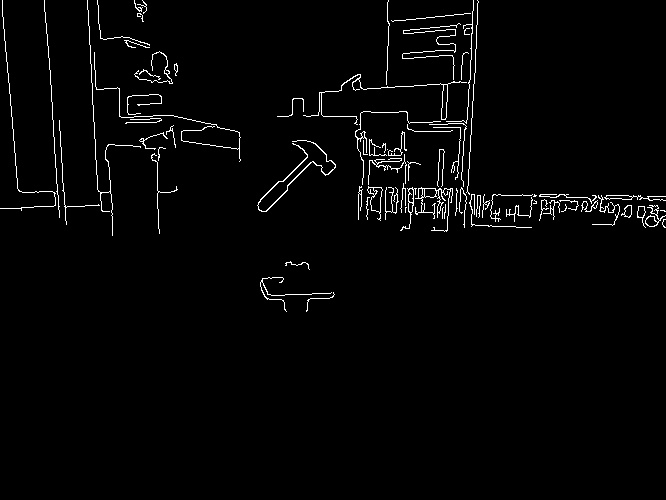
\includegraphics[width=1.0\textwidth]{img/piktogrammerkennung/edge_hammer.jpg}
  \caption{Kantenerkennung des Hammers}
  \label{fig:edge-hammer}
  \end{minipage} 
  \hfill
  \begin{minipage}[t]{0.45\linewidth}
  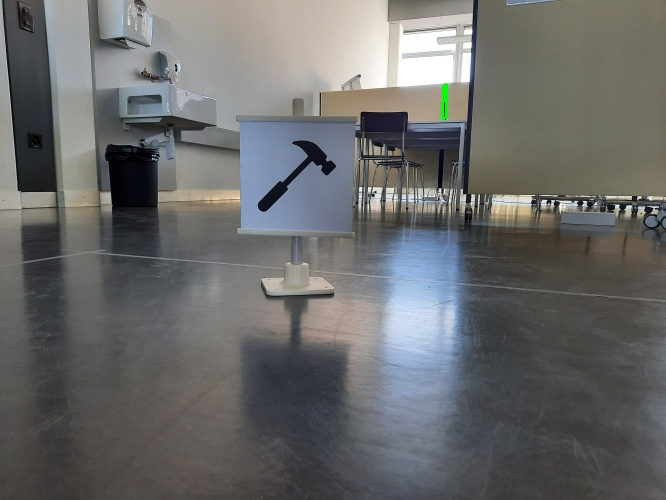
\includegraphics[width=1.0\textwidth]{img/piktogrammerkennung/contours_hammer.jpg}
  \caption{Erkannte Rechteckige Konturen des Hammers}
  \label{fig:contour-hammer}
  \end{minipage}
\end{figure}

Derselbe Algorithmus wurde an einem Beispielbild getestet, welches klare Kanten beinhaltet, welche steile Gradienten zur Folge haben. Auf dem nachfolgenden Bild \ref{fig:scanned-doc} sind die Resultate abgebildet. So konnte sichergestellt werden, dass der Algorithmus theoretisch zum gewünschten Ergebnis führt.

\begin{figure}[H]
  \centering
  \begin{minipage}[t]{0.32\linewidth}
  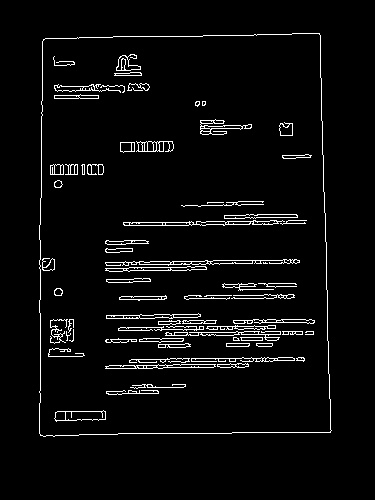
\includegraphics[width=1.0\textwidth]{img/piktogrammerkennung/edge_doc.jpg}
  \caption{Kantenerkennung des optimalen Testbildes}
  \label{fig:edge-doc}
  \end{minipage} 
  \hfill
  \begin{minipage}[t]{0.32\linewidth}
  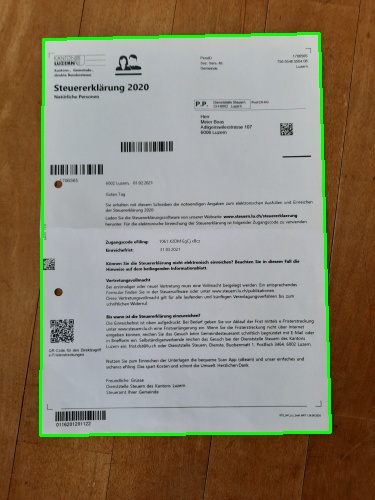
\includegraphics[width=1.0\textwidth]{img/piktogrammerkennung/contours_doc.jpg}
  \caption{Erkannte Rechteckige Konturen des optimalen Testbildes}
  \label{fig:contour-doc}
  \end{minipage}
  \hfill
  \begin{minipage}[t]{0.32\linewidth}
  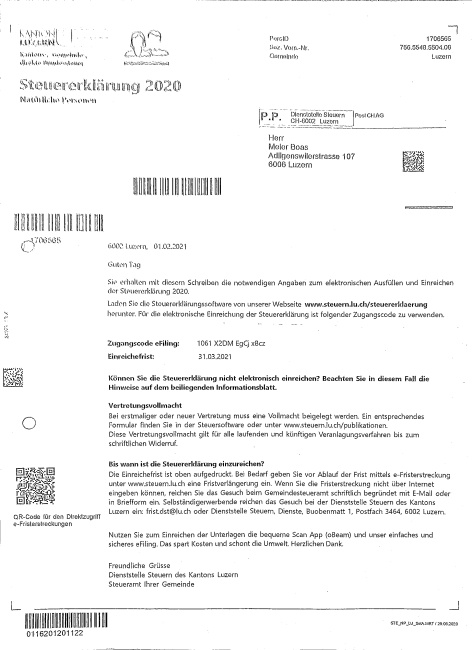
\includegraphics[width=1.0\textwidth]{img/piktogrammerkennung/scanned_doc.jpg}
  \caption{ROI Eingrenzung des optimalen Testbildes}
  \label{fig:scanned-doc}
  \end{minipage}
\end{figure}

\subsubsection{Bild für Detektion in Teilbilder aufteilen}
\label{sec:detektion-auf-teilbildern}
Da davon ausgegangen wurde, dass viel Hintergrundfläche einen negativen Einfluss auf die Matchergebnisse hat, war die Idee, das Bild in mehere Teilbilder aufzuteilen. Auf den einzelnen Teilbildern werden dann die Keypunkte extrahiert. Diese Keypunkte werden anschliessend für die Deskription und das Matching auf das gesamte Bild abgetragen.

\begin{figure}[H]
  \centering
  \begin{minipage}[t]{0.22\linewidth}
  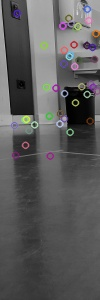
\includegraphics[width=1.0\textwidth]{img/piktogrammerkennung/slice0_kp2.jpg}
  \caption{Extrahierte Merkmale mit SIFT von Slice 0}
  \label{fig:slice0-kp2}
  \end{minipage} 
  \hfill
  \begin{minipage}[t]{0.22\linewidth}
  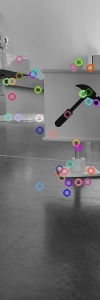
\includegraphics[width=1.0\textwidth]{img/piktogrammerkennung/slice1_kp2.jpg}
  \caption{Extrahierte Merkmale mit SIFT von Slice 1}
  \label{fig:slice1-kp2}
  \end{minipage}
  \hfill
  \begin{minipage}[t]{0.22\linewidth}
  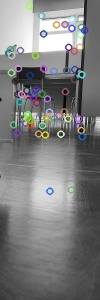
\includegraphics[width=1.0\textwidth]{img/piktogrammerkennung/slice2_kp2.jpg}
  \caption{Extrahierte Merkmale mit SIFT von Slice 2}
  \label{fig:slice2-kp2}
  \end{minipage}
  \hfill
  \begin{minipage}[t]{0.22\linewidth}
  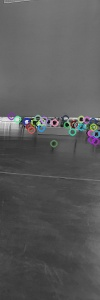
\includegraphics[width=1.0\textwidth]{img/piktogrammerkennung/slice3_kp2.jpg}
  \caption{Extrahierte Merkmale mit SIFT von Slice 3}
  \label{fig:slice3-kp2}
  \end{minipage}
\end{figure}

\begin{figure}[H]
  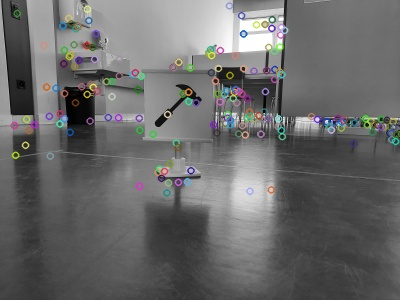
\includegraphics[width=0.95\textwidth]{img/piktogrammerkennung/sift_kp2_from_slice.jpg}
  \centering
  \caption{SIFT Merkmale der Slices auf das ursprüngliche Bild abgetragen}
  \label{fig:sift-kp2-slice}
\end{figure}

Um die Merkmale auf das uhrsprüngliche Bild zu übertragen, müssen zu deren x-Koordinaten in diesem Fall 100 px bzw. 200 px bzw. 300 px hinzuaddiert werden. Diese 100 px ergeben sich daraus, dass das Bild auf 400 px Breite skaliert wurde und in vier Streifen von je 100 px Breite geschnitten wurde. Hierbei hat sich gezeigt, dass sich die Werte beim anpassen teilweise sporadisch leicht ändern. 

Zum Beispiel hat sich zum Merkmal (6.106937408447266, 81.14856719970703) welches sich im zweiten Slice befindet 100 hinzuaddiert. Nach der Addition scheint der Wert noch zu stimmen: [106.10693740844727, 81.14856719970703]. Nach der Konvertierung in ein Tupel noch immer: (106.10693740844727, 81.14856719970703). Doch sobald die neue Koordinate effektiv dem \texttt{KeyPoint} zugewiesen wurde, stimmt der Wert ab der 6. Nachkommastelle nicht mehr überein: (106.10693359375, 81.14856719970703).

Bei anderen Merkmalen, scheint dies jedoch nicht der Fall zu sein:

(38.83573913574219, 117.7967529296875)\\
(138.8357391357422, 117.7967529296875)\\
(138.8357391357422, 117.7967529296875)\\
(138.8357391357422, 117.7967529296875)\\

Nachfolgend ein Auschnitt des Programmcodes, welcher zu den Keypunkten den entsprechenden Wert hinzuaddiert und von dem auch die obigen Koordinaten ausgegeben wurden:

\begin{minted}{python}
    for kp in kp2[1]:
        nkp = list(kp.pt)
        print(kp.pt)
        nkp[0] = nkp[0] + 100
        print(nkp)
        print(tuple(nkp))
        kp.pt = tuple(nkp)
        print(kp.pt)
    for kp in kp2[2]:
        nkp = list(kp.pt)
        nkp[0] = nkp[0] + 200
        kp.pt = tuple(nkp)
    for kp in kp2[3]:
        nkp = list(kp.pt)
        nkp[0] = nkp[0] + 300
        kp.pt = tuple(nkp)
    kp2 = list(chain.from_iterable(kp2))
\end{minted}

Aufjedenfall scheint sich diese sporadische Datenkorruption negativ auf die Matchergebnisse auszuwirken. In der Abbildung \ref{fig:sift-matches-slice} ist zu sehen, dass die gematchten Keypunkte nicht mehr zum Piktogramm gehören. 

\begin{figure}[H]
  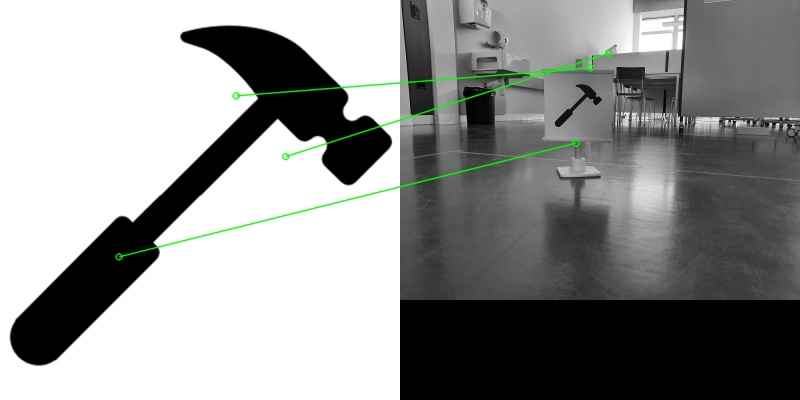
\includegraphics[width=0.95\textwidth]{img/piktogrammerkennung/sift_matches_slice.jpg}
  \centering
  \caption{Matches der SIFT Merkmale aus den verschiedenen Slices mit einem Matchverhältniss von 0.7}
  \label{fig:sift-matches-slice}
\end{figure}

Das oben geschilderte Problem wurde unter anderem nicht mehr weiter untersucht, da beim Auswerten der Anzahl guter Matches (siehe \ref{tab:sift-matchingresultate-image-slicing}) aufgefallen ist, dass sich diese in der Anzahl nicht unterscheiden. Ohne Slicing wurde die gleiche Anzahl Matches gefunden wie mit Slicing. Dies löste jedoch den Verdacht aus, \textbf{dass die gefundene Anzahl positiver Matches nicht von der Fläche des unrelevanten Hintergrundes abhängt, sondern von der Skalierung des Bildes!} Denn bei einem Zoom, beziehungsweise beim Wegschneiden des Hintergrundes wird nicht nur die Hintergrundfläche minimiert, sondern auch automatisch die Skalierung des Piktogramms verändert. Dies aus dem Grund, weil das Inputbild als auch das Template zu Beginn des Matchings auf 400 px breite skaliert wird.

\textbf{Matching Resultate}
\begin{center}
\begin{table}[H]
\begin{tabular}{|l|r|}
\hline
Keypoints 1 & 31 \\
\hline
Keypoints 2 & 218 \\
\hline
Matches & 31 \\
\hline
Good Matches & 3 \\
\hline
\end{tabular}
\caption[SIFT-Matchingresultate mit Image-Slicing]{SIFT-Matchingresultate mit Image-Slicing}
\label{tab:sift-matchingresultate-image-slicing}
\end{table}
\end{center}

\subsubsection{Skalierung}
Wie bereits am Ende des Kapitels \ref{sec:detektion-auf-teilbildern} beschrieben, kann es sein, dass nicht die Grösse der unrelevanten Hintergrundfläche die positiven Matches negativ beeinflussen, sondern die Skalierung des Piktogramm selber. Da beide Bilder auf 400 px Breite skaliert werden, ist das Piktogramm im Inputbild oftmals deutlich kleiner als das Piktogramm im Template. 

Im Bild \ref{fig:sift-matches-800} sind die Ergebnisse zu sehen, wenn das Inputbild auf 800 px Breite skaliert wird und nicht mehr auf 400 px wie das Template. Wie vermutet liefert SIFT deutlich bessere Ergebnisse, wenn der Skalierungsunterschied vom Template zum Objekt im Inputbild nicht zu gross ist. Obwohl es sich bei SIFT und ein Scale Invariantes Verfahren handelt, was so viel heisst wie, dass sich die Keypunkte und deren Deskriptoren aufgrund von Skalierung nicht verändern, werden bessere Resultate mit einer grösseren Skalierung des zu detektierenden Objektes erzielt. Der Grund dafür ist in den Matching Resultaten zu sehen. Bei einer Skalierung von 800 px werden deutlich mehr Keypunkte extrahiert. Die Chance auf eine grössere Anzahl positiver Matches steigt dementsprechend an.

\begin{figure}[H]
  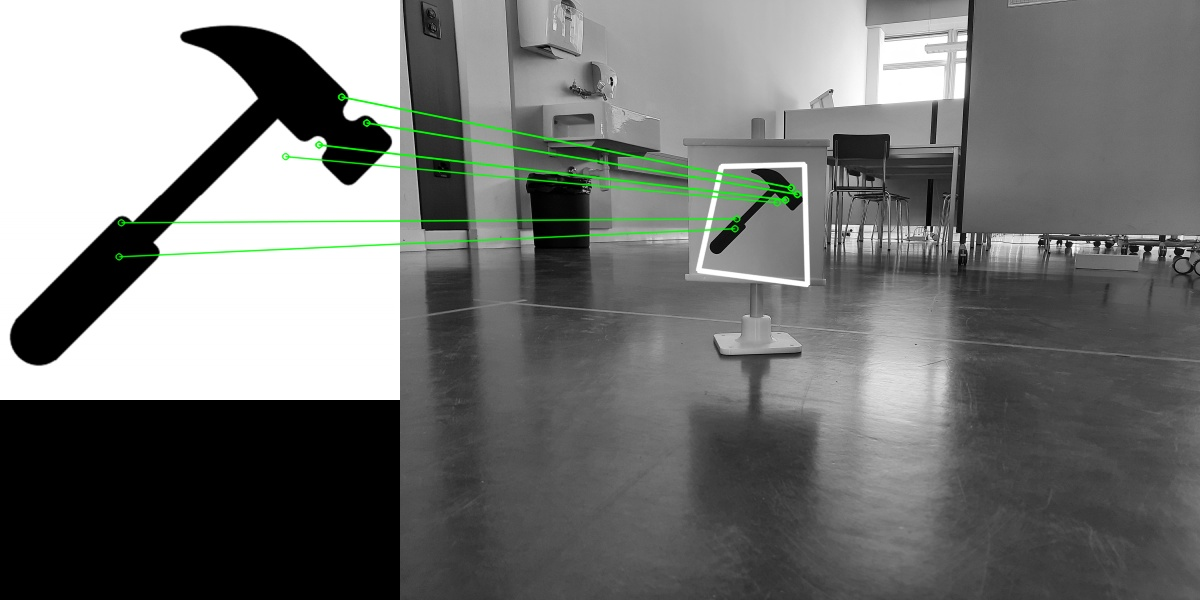
\includegraphics[width=0.95\textwidth]{img/piktogrammerkennung/sift_matches_800.jpg}
  \centering
  \caption{Matches der SIFT Merkmale bei einer Skalierung des Inputbildes auf 800px}
  \label{fig:sift-matches-800}
\end{figure}

\textbf{Matching Resultate}
\begin{center}
\begin{table}[H]
\begin{tabular}{|l|r|}
\hline
Keypoints 1 & 31 \\
\hline
Keypoints 2 & 400 \\
\hline
Matches & 31 \\
\hline
Good Matches & 13 \\
\hline
\end{tabular}
\caption[ORB-Matchingresultate]{ORB-Matchingresultate}
\label{tab:orb-matchingresultate}
\end{table}
\end{center}

\newpage

\subsection{Performance}
Die Laufzeit des Feature Matchings konnte fast halbiert werden, in dem die Features der zu detektierenden Piktogramme bereits in der Initialisierungsphase extrahiert werden. Ebenfalls in der Initialisierungsphase werden bereits die Deskriptoren berechnet und abgespeichert. Während des eigentlichen Laufes müssen also nur noch die Feautures und Deskriptoren des Input-Bildes berechnet werden und mit den bereits vorberechneten Deskriptoren abgeglichen werden.

Weitere Performance-Tests oder -Optimierungen wurden nicht mehr vorgenommen, da der Feature Matching Algorithmus auf dem Jetson Nano in wenigen Millisekunden durchlaufen werden kann.  






